\section{Data}
\label{sec:data}
The data were collected from the public part of the HackerOne website. From 35 public bounty programs, we collected the rewards received by security researchers (in US dollars), with their timestamps (45 other public bounty programs do not disclose detailed information on rewards, and the number of private programs is not disclosed). Since HackerOne started its platform in December 2013, new public programs have been launched roughly every two months, following an essentially memoryless Poisson process ($\lambda = 57$ days, $p < 0.001$ and $R^2 > 0.99$). Figure \ref{timeline}A shows the timeline of the 9 most active programs with at least 90 valid (i.e., rewarded) bug discoveries, as of February 15th, 2016. When a new program is launched, we observe an initial peak within weeks after launch, which accounts for the majority of discoveries. After the initial surge of vulnerability discoveries, bounty awards become less frequent following a robust power law decay $\sim t^{\alpha}$ with $\alpha = -0.40(4)$ ($p < 0.001$ and $R^2 = 0.79$; the fit of the time series was obtained using ordinary least square regression as described in \cite{maillart2011quantification}) at the aggregate level and over all 35 bounty programs (see Figure \ref{timeline}B). Some programs depart from this averaged trend: For instance, Twitter exhibits a steady, almost constant, bug discovery rate and VKontakte exhibits its peak activity months after the initial launch. These peculiar behaviors may be attributed to program tuning and marketing, to sudden change of media exposure or even to fundamental differences of program comparative fitness, for which we do not have specific information.\\

\begin{figure}[h]
\begin{center}
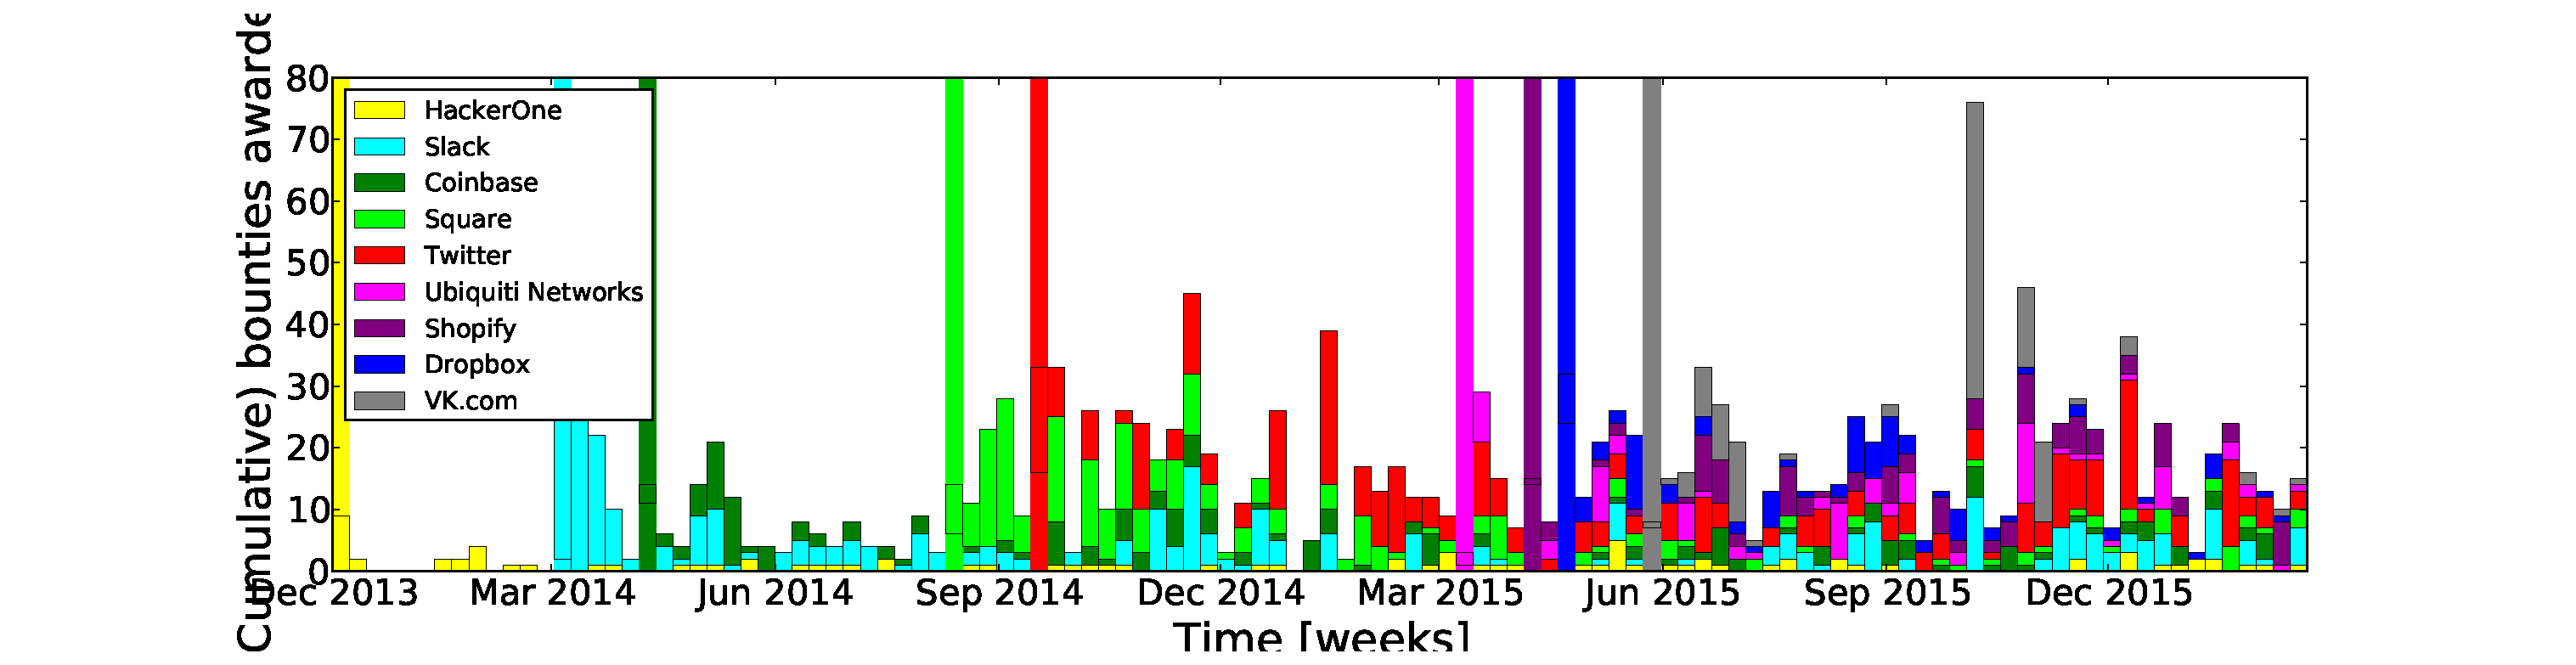
\includegraphics[width=12cm]{../figures/timeline.eps}
\caption{\footnotesize {\bf A.} Weekly vulnerability discoveries for the 9 most active programs (with at least 90 bug discoveries as of February 15, 2016). The light colored vertical bars represent the start of the program, occurring when the first bounty is awarded. Most programs exhibit an initial shock, followed by a decay of discoveries, which is characterized at the aggregate level by a long-memory process (panel {\bf B}) characterized by a power law decay $\sim t^{\alpha}$ with $\alpha = -0.40(4)$ ($p < 0.001$ and $R^2 = 0.79$, obtained by ordinary least square fitting). Each data point in the figure is the median of normalized vulnerability numbers of all 35 programs considered in this study.}
\label{timeline}
\end{center}
\end{figure}

The power law decay observed here is reminiscent of the long-established $\sim 1/\tau$ law of bug discovery in software testing \cite{adams1984textordfeminineoptimizing}. This similitude is interesting even though bug bounty programs do not provide direct information regarding software reliability. The difference of exponent ($\alpha \approx 0.4$ instead of $1$), may stem from long-memory processes associated with human behaviors and human timing effects, which correspond to task priority queueing and a rationale use of time as non-storable scarce resource \cite{maillart2011quantification}. Long-memory processes observed in collective human behaviors such as those observed on Figure \ref{timeline}B may also be associated with critical cascades of productive events \cite{sornette2014much}. The intuition is that each security researcher will generate a cascade of bug discoveries (of a size related to the total number of bugs discovered by this person, which is a random variable across all researchers), and by her activity (each researcher will influence and attract other researchers), hence generating cascades of joining and of bug discoveries.\\

%Here, the rationale for cascades builds on 2 ingredients : (i) each security researcher generates a cascade of bug discoveries, and (ii) each bug discovery attracts new security researchers, who in turn trigger their own bug discovery cascade. Cascades are typically slightly heavy-tailed, however bounded, as we'll later : we will dissect these cascades in conjunction with incentives provided by the accumulation of bounties (reputation, slight chance to find less obvious bugs bring more reputation, and increased bounties rewards)}.

Here, we do not consider the human timing effects encompassing delays, effort, processing time, and influence. We only consider incremental valid bug discovery and reporting by security researchers.

